\documentclass{article}

\usepackage[utf8]{inputenc}
\usepackage{longtable}
\usepackage{authblk}
\usepackage{adjustbox}

\usepackage{natbib}


\title{LOS INDICES DE COLOMBIA}
% autores
\renewcommand\Authand{ y }
\author[1]{\normalsize Nicolas Alvarez}

\affil[1]{\small  Universidad de los Andes\\
\texttt{{nd.alvarez11}@uniandes.edu.col}}

\date{29 de Junio de 2018}

\usepackage{Sweave}
\begin{document}
\Sconcordance{concordance:Proyecto.tex:Proyecto.Rnw:%
1 20 1 1 0 23 1 1 13 3 1 1 10 14 0 1 3 8 1 1 4 1 3 9 1 1 8 1 3 8 1 1 11 %
1 3 11 1 1 5 12 0 1 2 3 1 1 9 13 0 1 2 8 1 2 2 12 1 1 5 1 1 1 4 31 0 1 %
2 13 1 1 11 1 16 3 1 1 8 3 0 1 2 5 0 1 16 1 0 1 3 10 1}


\maketitle

\begin{abstract}
Este es mi primer trabajo en exploracion y modelamiento de indices usando LATEX. Este trabajo lo he hecho bajo la filosofia de trabajo replicable. Este es mi primer trabajo en exploracion y modelamiento de indices usando LATEX. Este trabajo lo he hecho bajo la filosofia de trabajo replicable. Este es mi primer trabajo en exploracion y modelamiento de indices usando LATEX. Este trabajo lo he hecho bajo la filosofia de trabajo replicable. Este es mi primer trabajo en exploracion y modelamiento de indices usando LATEX. Este trabajo lo he hecho bajo la filosofia de trabajo replicable.
\end{abstract}


\section*{Introduccion}

Aqui les presento mi investigacion sobre diversos indices sociales en el mundo. Los indices los consegui de wikipedia, espero que les gusten mucho. Aqui les presento mi investigacion sobre diversos indices sociales en el mundo. Los indices los consegui de wikipedia, espero que les gusten mucho.Aqui les presento mi investigacion sobre diversos indices sociales en el mundo. Los indices los consegui de wikipedia, espero que les gusten mucho.Aqui les presento mi investigacion sobre diversos indices sociales en el mundo. Los indices los consegui de wikipedia, espero que les gusten mucho.
Aqui les presento mi investigacion sobre diversos indices sociales en el mundo. Los indices los consegui de wikipedia, espero que les gusten mucho.Aqui les presento mi investigacion sobre diversos indices sociales en el mundo. Los indices los consegui de wikipedia, espero que les gusten mucho.Aqui les presento mi investigacion sobre diversos indices sociales en el mundo. Los indices los consegui de wikipedia, espero que les gusten mucho.

Comencemos viendo que hay en la seccion \ref{univariada} en la pagina \pageref{univariada}.

\clearpage

\section{Exploracion Univariada}\label{univariada}

En esta seccion exploro cada indice. En esta seccion exploro cada indice. En esta seccion exploro cada indice. En esta seccion exploro cada indice. En esta seccion exploro cada indice. En esta seccion exploro cada indice. En esta seccion exploro cada indice. En esta seccion exploro cada indice. En esta seccion exploro cada indice.


\begin{Schunk}
\begin{Soutput}
'data.frame':	32 obs. of  6 variables:
 $ IDH              : num  0.879 0.867 0.865 0.849 0.842 0.839 0.837 0.835 0.834 0.832 ...
 $ Departamento     : chr  "Santander" "Casanare" "Valle del Cauca" "Antioquia" ...
 $ PoblacionCabecera: int  1587972 281548 4169553 5262172 742812 761658 10070801 2438533 56487 506254 ...
 $ PoblacionResto   : int  502867 93701 586560 1428858 539251 206109 914484 107391 21926 68756 ...
 $ PoblacionTotal   : int  2090839 375249 4756113 6691030 1282063 967767 10985285 2545924 78413 575010 ...
 $ DepartamentoNorm : chr  "Santander" "Casanare" "Valle del Cauca" "Antioquia" ...
\end{Soutput}
\end{Schunk}

Este es el comportamiento de las variables a estudiar. Veamos su tabla de frecuencias:


% Table created by stargazer v.5.2.2 by Marek Hlavac, Harvard University. E-mail: hlavac at fas.harvard.edu
% Date and time: vie., jun. 29, 2018 - 7:22:51 p. m.
\begin{table}[!htbp] \centering 
  \caption{Medidas estadisticas} 
  \label{stats} 
\begin{tabular}{@{\extracolsep{5pt}}lcccccc} 
\\[-1.8ex]\hline 
\hline \\[-1.8ex] 
Statistic & \multicolumn{1}{c}{N} & \multicolumn{1}{c}{Mean} & \multicolumn{1}{c}{St. Dev.} & \multicolumn{1}{c}{Median} & \multicolumn{1}{c}{Min} & \multicolumn{1}{c}{Max} \\ 
\hline \\[-1.8ex] 
IDH & 32 & 0.802 & 0.042 & 0.804 & 0.691 & 0.879 \\ 
PoblacionCabecera & 32 & 1,196,730.000 & 1,982,287.000 & 717,197 & 13,090 & 10,070,801 \\ 
PoblacionResto & 32 & 360,590.300 & 331,887.600 & 268,111.5 & 21,926 & 1,428,858 \\ 
\hline \\[-1.8ex] 
\end{tabular} 
\end{table} 

graficos

%%%%% figure
\begin{figure}[h]
\centering
\begin{adjustbox}{width=5cm,height=5cm,clip,trim=1.5cm 0.5cm 0cm 1.5cm}
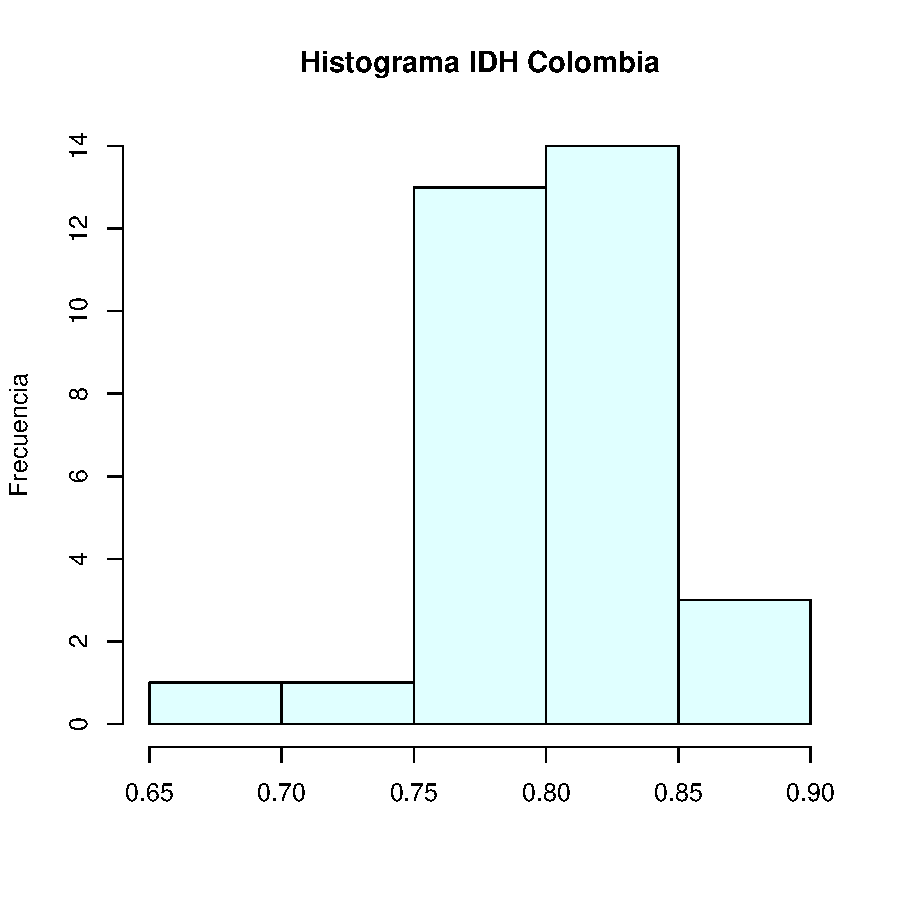
\includegraphics{Proyecto-003}
\end{adjustbox}
\caption{Histograma de IDH}
\label{histogramaIDH}
\end{figure}


%%%%% figure
\begin{figure}
\centering
\begin{adjustbox}{width=7cm,height=7cm,clip,trim=1.5cm 0.5cm 0cm 1.5cm}
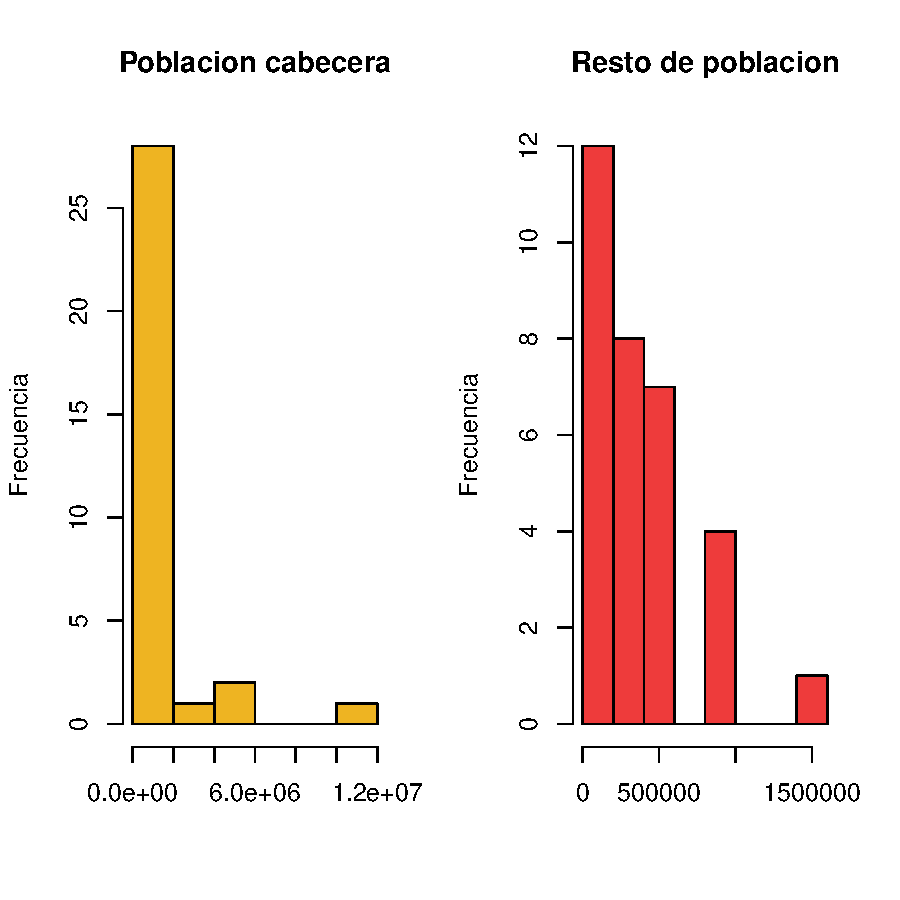
\includegraphics{Proyecto-004}
\end{adjustbox}
\caption{Histogramas de poblacion diferenciando de la cabecera municipal y el resto de la poblacion}
\label{histogramaPobla}
\end{figure}

%%%%% figure
\begin{figure}
\centering
\begin{adjustbox}{width=7cm,height=7cm,clip,trim=1.5cm 0.5cm 0cm 1.5cm}
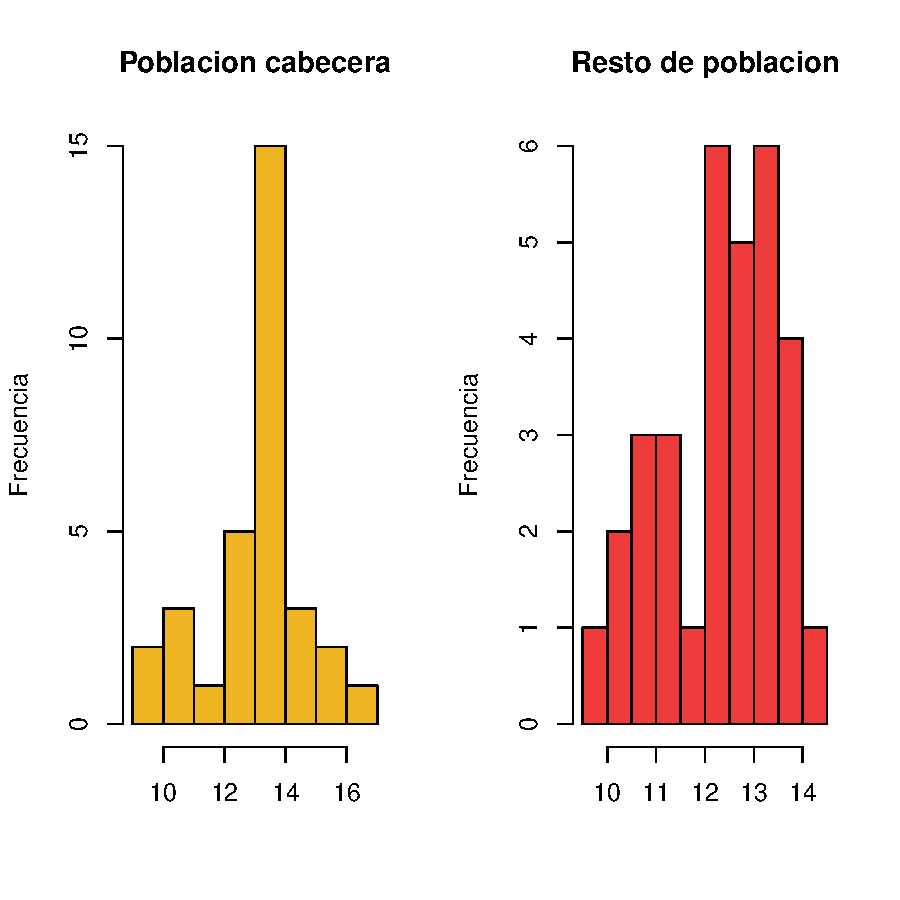
\includegraphics{Proyecto-005}
\end{adjustbox}
\caption{Histogramas de poblacion diferenciando de la cabecera municipal y el resto de la poblacion normalizda}
\label{histogramaPoblaNorm}
\end{figure}

\clearpage


\section{Exploracion Bivariada}

En este trabajo estamos interesados en el impacto de los otros indices en el nivel de Democracia. Veamos las relaciones bivariadas que tiene esta variable con todas las demas:

% Table created by stargazer v.5.2.2 by Marek Hlavac, Harvard University. E-mail: hlavac at fas.harvard.edu
% Date and time: vie., jun. 29, 2018 - 7:23:02 p. m.
\begin{table}[!htbp] \centering 
  \caption{Correlacion de IDH con las poblaciones} 
  \label{corrIDH} 
\begin{tabular}{@{\extracolsep{5pt}} cc} 
\\[-1.8ex]\hline 
\hline \\[-1.8ex] 
PoblacionCabeceraLog & PoblacionRestoLog \\ 
\hline \\[-1.8ex] 
$0.487$ & $0.177$ \\ 
\hline \\[-1.8ex] 
\end{tabular} 
\end{table} 

Veamos la correlacion entre las variables independientes:

% Table created by stargazer v.5.2.2 by Marek Hlavac, Harvard University. E-mail: hlavac at fas.harvard.edu
% Date and time: vie., jun. 29, 2018 - 7:23:02 p. m.
\begin{table}[!htbp] \centering 
  \caption{Correlacion entre variables independientes} 
  \label{corrTableX} 
\begin{tabular}{@{\extracolsep{5pt}} ccc} 
\\[-1.8ex]\hline 
\hline \\[-1.8ex] 
 & PoblacionCabeceraLog & PoblacionRestoLog \\ 
\hline \\[-1.8ex] 
PoblacionCabeceraLog & 1 &  \\ 
PoblacionRestoLog & 0.84 & 1 \\ 
\hline \\[-1.8ex] 
\end{tabular} 
\end{table} 

Lo visto en la Tabla \ref{corrTableX} se refuerza claramente en la Figura \ref{corrPlotX}.



\begin{figure}[h]
\centering
\begin{adjustbox}{width=7cm,height=7cm,clip,trim=1.5cm 0.5cm 0cm 1.5cm}
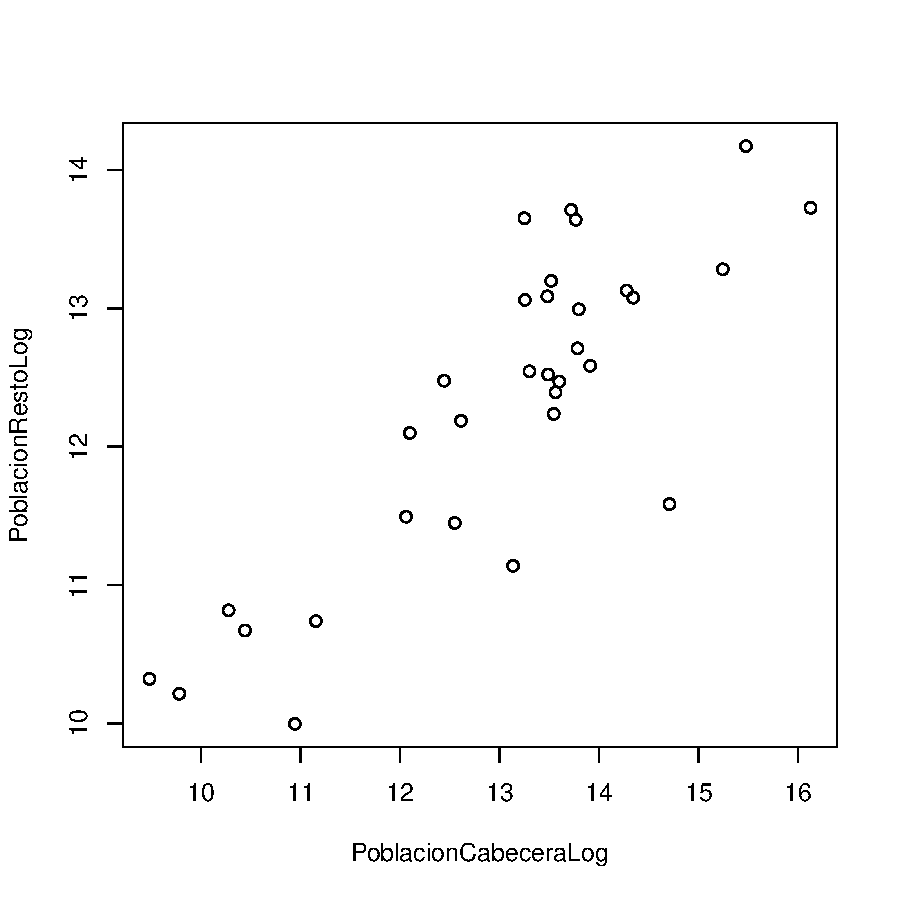
\includegraphics{Proyecto-corrPlotX}
\end{adjustbox}
\caption{correlacion entre predictores}
\label{corrPlotX}
\end{figure}

\clearpage


\section{Modelos de Regresion}

Finalmente, vemos los modelos propuestos. Primero sin la resto de poblacion como independiente, y luego con esta. Los resultados se muestran en la Tabla \ref{regresiones} de la pagina \pageref{regresiones}.




% Table created by stargazer v.5.2.2 by Marek Hlavac, Harvard University. E-mail: hlavac at fas.harvard.edu
% Date and time: vie., jun. 29, 2018 - 7:23:02 p. m.
\begin{table}[!htbp] \centering 
  \caption{Modelos de Regresion} 
  \label{regresiones} 
\begin{tabular}{@{\extracolsep{5pt}}lcc} 
\\[-1.8ex]\hline 
\hline \\[-1.8ex] 
 & \multicolumn{2}{c}{\textit{Dependent variable:}} \\ 
\cline{2-3} 
\\[-1.8ex] & \multicolumn{2}{c}{IDH} \\ 
\\[-1.8ex] & (1) & (2)\\ 
\hline \\[-1.8ex] 
 PoblacionCabeceraLog & 0.013$^{***}$ & 0.031$^{***}$ \\ 
  & (0.004) & (0.007) \\ 
  & & \\ 
 PoblacionRestoLog &  & $-$0.030$^{***}$ \\ 
  &  & (0.010) \\ 
  & & \\ 
 Constant & 0.634$^{***}$ & 0.766$^{***}$ \\ 
  & (0.055) & (0.065) \\ 
  & & \\ 
\hline \\[-1.8ex] 
Observations & 32 & 32 \\ 
R$^{2}$ & 0.238 & 0.425 \\ 
Adjusted R$^{2}$ & 0.212 & 0.385 \\ 
Residual Std. Error & 0.037 (df = 30) & 0.033 (df = 29) \\ 
F Statistic & 9.347$^{***}$ (df = 1; 30) & 10.706$^{***}$ (df = 2; 29) \\ 
\hline 
\hline \\[-1.8ex] 
\textit{Note:}  & \multicolumn{2}{r}{$^{*}$p$<$0.1; $^{**}$p$<$0.05; $^{***}$p$<$0.01} \\ 
\end{tabular} 
\end{table} 
Como se en la Tabla \ref{regresiones}, cuando esta presente el \emph{resto de la poblacion}, el \emph{el factor de resto de la poblacion} pierde significancia.


\clearpage


\section{Exploracion Espacial}

Como acabamos de ver en la Tabla \ref{regresiones} en la pagina \pageref{regresiones}, si quisieras sintetizar la multidimensionalidad de nuestros indicadores, podriamos usar tres de las cuatro variables que tenemos (un par de las originales tiene demasiada correlacion). 

AsÃ<U+00AD>, propongo que calculemos conglomerados de paÃ<U+00AD>ses usando toda la información de tres de los indicadores. Como nuestras variables son ordinales utilizaremos un proceso de conglomeración donde las distancia serán calculadas usando la medida {\bf macqueen} propuestas en \cite{macqueen_methods_nodate}. Los tres conglomerados se muestran en la Figura \ref{clustmap}.




\begin{figure}[h]
\centering
%\begin{adjustbox}{width=11cm,height=8cm,clip,trim=1cm 2.5cm 0cm 2.5cm}
\begin{Schunk}
\begin{Soutput}
[1] 2 1 3
\end{Soutput}
\begin{Soutput}
  Group.1       IDH PoblacionCabeceraLog PoblacionRestoLog
1       1 0.8183684             14.04629          12.98461
2       2 0.7525556             11.28126          11.39788
3       3 0.8342500             12.17091          11.01873
\end{Soutput}
\end{Schunk}
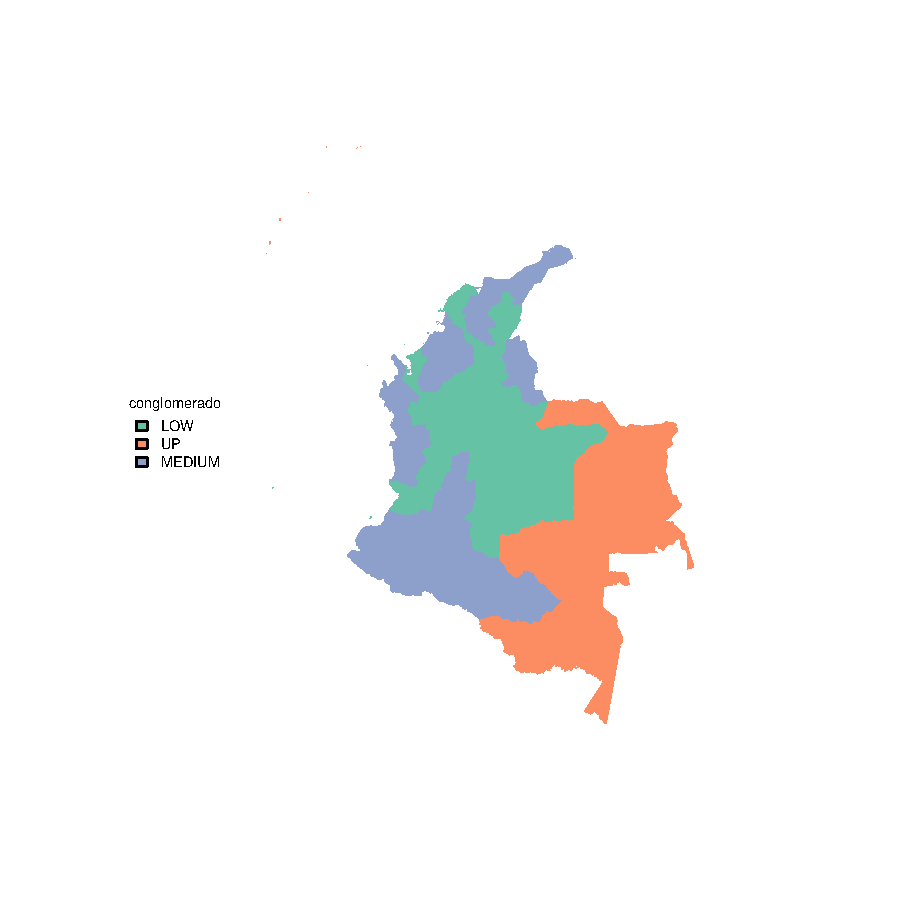
\includegraphics{Proyecto-plotMap1}
%\end{adjustbox}
\caption{Paises conglomerados segun sus indicadores sociopoliticos}\label{clustmap}
\end{figure}

\bibliographystyle{apalike}
\renewcommand{\refname}{Bibliografia}
\bibliography{Proyecto}



\end{document}
